\documentclass[a4paper,12pt]{article}

\title{Biology 30 IB \\ Genetics}
\author{Jad Chehimi}

% document setup
\renewcommand{\familydefault}{\sfdefault}
\linespread{1.25}
\usepackage[margin=1in]{geometry}
\usepackage{setspace}
\usepackage{enumitem}
\setlist{nosep}
\usepackage{color,soul}
\setcounter{secnumdepth}{0}

% tools
\usepackage[hidelinks]{hyperref}
\usepackage{float}
%% images
\usepackage{graphicx}
\graphicspath{ {./images/} }
%% science
\usepackage{siunitx}

\begin{document}
\maketitle

\tableofcontents

\pagebreak

\section{(18.1) Gregor Mendel}
\begin{itemize}
    \item{Created the \hl{Laws of Inheritance of Traits}}
    \item{Studied inheritance of traits in \hl{pea plants} (test question)}
    \item{Called DNA and chromosomes particles --- he didn't know}
    \item{\hl{Father of Genetics}}
\end{itemize}

\subsection{Peas}
\begin{itemize}
    \item{Can be grown in a small area}
    \item{Produce lots of offspring}
    \item{Self-pollinate}
    \item{Can be \hl{artificially cross-pollinated} (test question)}
\end{itemize}

\section{Introduction}
\subsection{General}
\begin{itemize}
    \item{\textbf{Trait} = any \hl{characteristic} that can be passed from \hl{parent to offspring}}
    \item{\textbf{Heredity} = passing of traits from parent to offspring}
    \item{\textbf{Genetics} = study of heredity}
\end{itemize}

\subsection{Terms}
\begin{itemize}
    \item{\textbf{Alleles} = two forms of a gene --- \hl{dominant \& recessive}}
    \item{\textbf{Dominant} = \hl{stronger} of two genes, represented with \hl{capital letter} (R)}
    \item{\textbf{Recessive} = \hl{weaker} of two genes, represented with \hl{lowercase letter} (r)}
    \item{\textbf{Genotype} = gene combination for a trait (\hl{RR, Rr, rr}) separated with colons}
    \item{\textbf{Phenotype} = \hl{physical feature} resulting from genotype (red, white) separated with colons}
    \item{\textbf{Homozygous genotype} = genotype involving \hl{2 dominant} OR \hl{2 recessive} genes --- \hl{pure}, RR or rr}
    \item{\textbf{Heterozygous genotype} = genotype involving \hl{1 dominant} OR \hl{1 recessive} gene --- \hl{hybrid}, Rr}
\end{itemize}

\pagebreak

\subsubsection{Dominance}
\begin{itemize}
    \item{Dominant and recessive alleles can code for different things}
    \item{e.x. R = Brown eyes, r = blue eyes}
    \item{\hl{Any dominant alleles} = \hl{dominant phenotype} --- RR, Rr in most cases}
    \item{\hl{Only recessive alleles} = \hl{recessive phenotype} --- rr}
\end{itemize}

\begin{figure}[H]
    \centering
    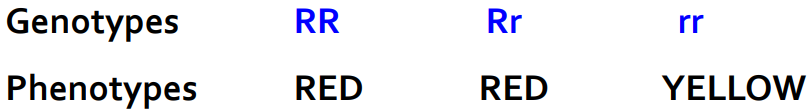
\includegraphics[width=0.75\textwidth]{dom}
\end{figure}

\subsubsection{Crosses}
\begin{itemize}
    \item{\textbf{Monohybrid cross} = cross involving a single trait}
    \item{\textbf{Dihybrid cross} = cross involving two traits}
    \item{\textbf{Test cross} = cross involving always involing a \hl{homozygous recessive (rr)} parent crossed with an unknown genotype, in order to \hl{find the genotype}}
\end{itemize}

\subsubsection{Generations}
\begin{itemize}
    \item{\textbf{P1 Generation} = parental generation in a breeding experiment}
    \item{\textbf{F1 Generation} (1st filial gen) = first-generation offspring in a breeding experiment}
    \item{\textbf{F2 Generation} (2nd filial gen) = second-generation offspring, and so on...}
\end{itemize}

\section{Mendel's Laws}
\begin{figure}[H]
    \centering
    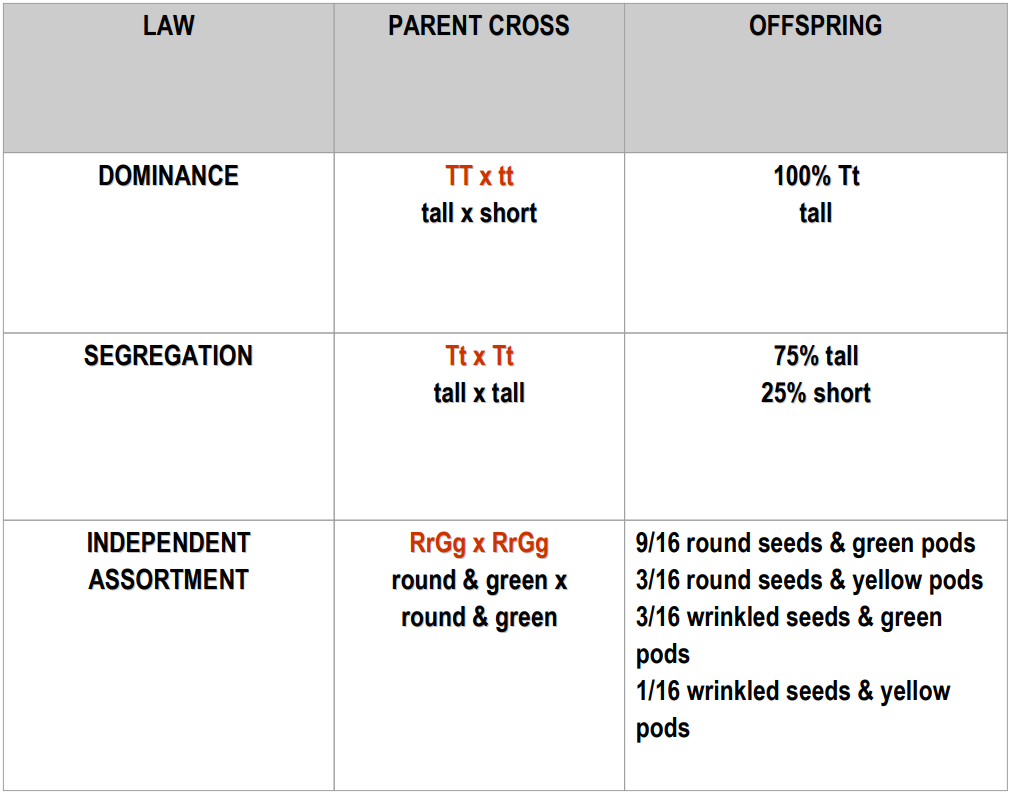
\includegraphics[width=0.75\textwidth]{laws}
\end{figure}

\section{(18.2) Punnett Squares}
\begin{figure}[H]
    \centering
    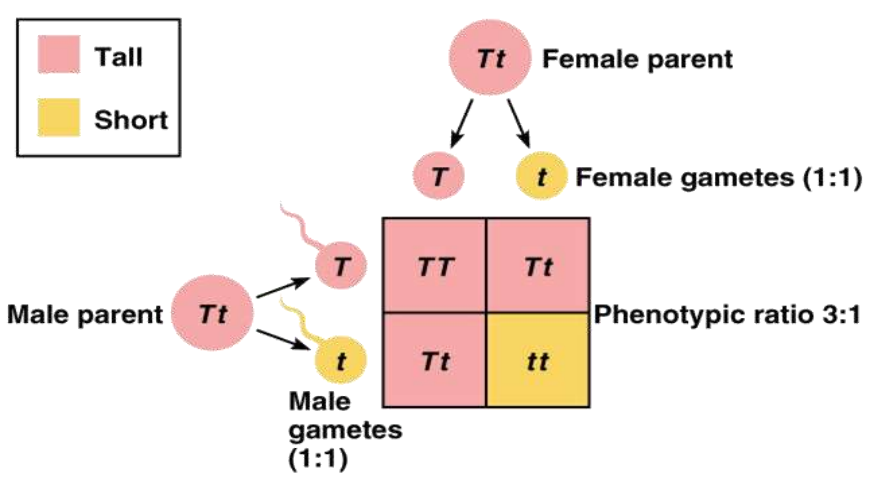
\includegraphics[width=\textwidth]{punnett}
    \caption{Punnett square demonstrating \hl{law of segregation}, which occurs in \hl{anaphase I}}
\end{figure}
\begin{itemize}
    \item{One gene from father, one gene from mother}
    \item{Dominant and recessive alleles compete in punnett squares}
    \item{\textbf{Phenotypic ratio} = ratio of \hl{dominant phenotypes to recessive phenotypes}, in this diagram its \texttt{3:1}}
\end{itemize}

\section{(18.3) Pedigree Charts}
\begin{figure}[H]
    \centering
    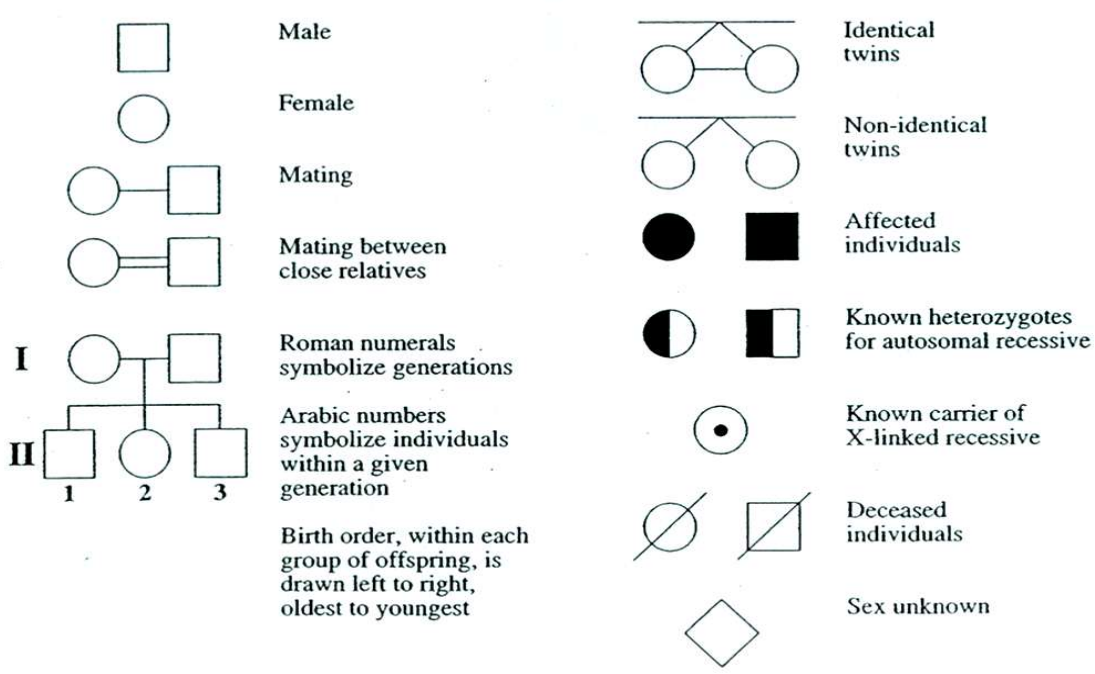
\includegraphics[width=0.9\textwidth]{pedigree}
    \caption{All in your data booklet, \hl{except known heterozygotes}}
\end{figure}
\begin{itemize}
    \item{\textbf{Pedigree} = a family tree used to \hl{trace inherited traits} from parents to offspring}
    \item{Roman numerals denote different generations (rows)}
    \item{Arabic numerals denote different individuals in a generation (columns)}
\end{itemize}

\subsection{Terms}
\begin{itemize}
    \item{\textbf{Autosomal condition} = \hl{almost equal} number of males and females are affected by a condition}
    \item{\textbf{Dominance condition} = condition \hl{appears in every} generation}
    \item{\textbf{Recessive condition} = condition \hl{does not} appear in every generation; skips generations}
\end{itemize}

\section{(18.4) Other Patterns of Inheritance}

\subsection{Pleiotropy}
\begin{itemize}
    \item{\textbf{Pleiotropic gene} = one gene \hl{affects more than one} phenotypic characteristic}
    \item{
            Examples of wide-ranging effects from a single gene include...
            \begin{itemize}
                \item{dwarfism (achondroplasia)}
                \item{gigantism (acromegaly)}
\end{itemize}
        }
\end{itemize}

\subsection{Multiple Alleles}
\begin{itemize}
    \item{Possible to have more than two alleles for a trait}
    \item{Superscript identifies different alleles}
    \item{
            Different alleles are dominant to one another
            \begin{itemize}
                \item{e.g. $E^1 > E^2 > E^3 > E^4$}
            \end{itemize}
        }
\end{itemize}

\subsubsection{Example}
Predict the genotypic and phenotypic outcomes of crossing $E^1E^4 \times E^2E^3$.

\begin{itemize}
    \item{$E^1$ = wild, $E^2$ = apricot, $E^3$ = honey, $E^4$ = white}
\end{itemize}

\begin{figure}[H]
    \centering
    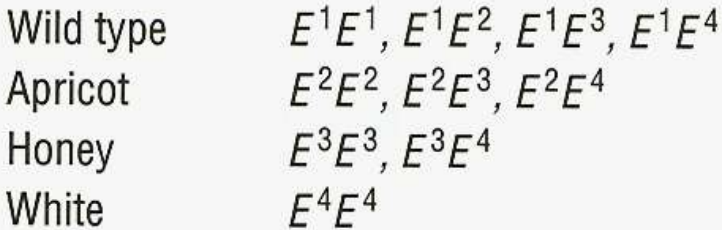
\includegraphics[width=0.50\textwidth]{ex1a}
    \caption{This is typically given}
\end{figure}

\begin{figure}[H]
    \centering
    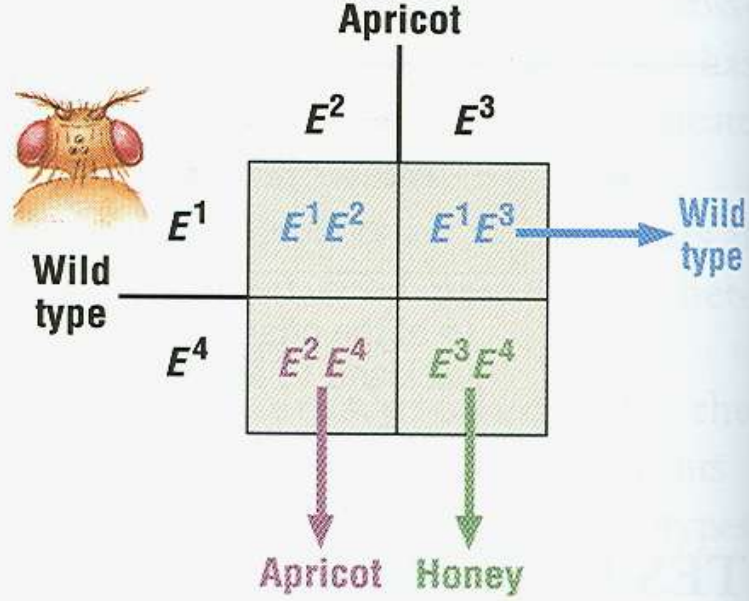
\includegraphics[width=0.50\textwidth]{ex1b}
\end{figure}

\begin{itemize}
    \item{Genotype = $1 \times E^1E^2 : 1 \times E^1E^3 : 1 \times E^2E^4 : 1 \times E^3E^4$}
    \item{Phenotype = 2 wild : 1 apricot : 1 honey}
\end{itemize}

\subsection{Incomplete Dominance}
\begin{itemize}
    \item{A hybrid (Rr) appearance can sometimes be \hl{in between the phenotypes}}
    \item{
            For example...
            \begin{itemize}
                \item{RR = red}
                \item{rr = white}
                \item{Rr = \hl{pink} (normally red)}
            \end{itemize}
        }
\end{itemize}

\subsection{Codominance}
\begin{itemize}
    \item{\hl{Both alleles expressed in heterozygous individuals}}
\end{itemize}

\begin{figure}[H]
    \centering
    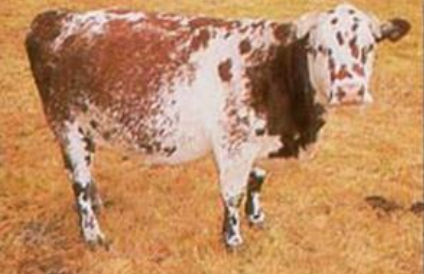
\includegraphics[width=0.50\textwidth]{codom}
    \caption{Red bull + white cow = red and white hair}
\end{figure}

\subsection{Blood Type}
Example of codominance and multiple alleles

$I^A$ \& $I^B$ $>$ $i$
\begin{itemize}
    \item{Type A = $I^AI^A$ or $I^Ai$}
    \item{Type B = $I^BI^B$ or $I^Bi$}
    \item{Type AB = $I^AI^B$}
    \item{Type O = $ii$}
\end{itemize}

\pagebreak

\section{(18.5) Dihybrid Crosses}
\begin{itemize}
    \item{A breeding experiment that tracks the inheritance of \hl{two traits}}
    \item{\textbf{Law of Independent Assortment} = each pair of alleles segregate independently (metaphase)}
    \item{The two traits \hl{do not influence one another}, they are independent}
    \item{These traits are on different locations --- called \textbf{loci}, \textbf{locus} --- of a chromosome}
\end{itemize}

\subsection{\# of Unique Gametes}\noindent

\begin{center}
\Huge $2^n$ \normalsize

$n$ = \# of heterozygotes of \hl{each parent}
\end{center}

Examples...
\begin{itemize}
    \item{\underline{RrBb} = 2 heterozygotes = $2^2 = 4$ gametes}
    \item{yypp = 0 heterozygotes = $2^0 = 1$ gamete}
    \item{\underline{AaBb}CC\underline{Dd} = 3 heterozygotes = $2^3 = 8$ gametes}
    \item{\underline{MmNnOo}PPQQ\underline{Rr}ss\underline{TtXx} = 6 heterozygotes = $2^6 = 64$ gametes}
\end{itemize}

\subsection{Drawing a Dihybrid Cross}
Determine how many different possible gametes/phenotypes with the formula.
\begin{itemize}
    \item{$2^2$ = 4}
    \item{There will be 4 different types of offspring from this cross}
    \item{If a question specifically asks for the \hl{adults}, there may be a gene that prevents adulthood --- i.e. a fatal gene --- so do not include that combination in any percent calculations and ratios}
    \item{If you are doing a test cross --- there is an unknown gene --- make a dihybrid cross for each possible combination; this applies to monohybrid aswell}
        \\
\end{itemize}

\pagebreak

Prepare a cross for every possible combination of all heterozygotes.
\begin{enumerate}
    \item{Top header = \hl{FOIL} between genes of the gene pair of the first parent}
    \item{Left header = \hl{FOIL} between genes of the gene pair of other parent}
    \item{You can skip redundent combinations}
    \item{Fill in the table like usual, including the top and left header, to list every possible combination}
    \item{Make sure to order the alleles dominant to recessive, and same letters together}
\end{enumerate}

Using the cross, you can...
\begin{itemize}
    \item{Determine the number/ratio of all possible genotypes by counting}
    \item{Determine the number of phenotypes from all possible genotypes}
\end{itemize}
It helps to mark each of the table cells with a symbol to keep track.

\subsubsection{Example}
\begin{itemize}
    \item{R\_ = round, Y\_ = yellow}
    \item{rr = wrinkled, yy = green}
\end{itemize}

Question: Determine the genotype and phenotype of a RyYy x RyYy cross.

\begin{figure}[H]
    \centering
    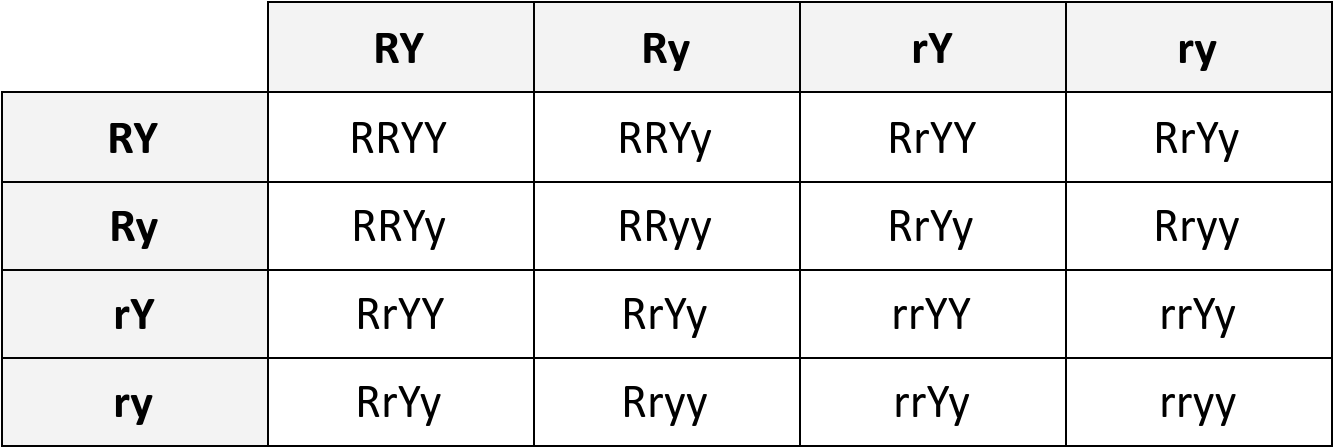
\includegraphics[width=\textwidth]{dihybrid}
\end{figure}

\begin{itemize}
    \item{Genotype \\ $1 \times RRYY : 2 \times RRYy : 2 \times RrYY : 4 \times RrYy : 1 \times RRyy : 2 \times Rryy : 1 \times rrYY : 2 \times rrYy : 1 \times rryy$}
    \item{
            Phenotype
            \begin{itemize}
                \item{9 round, yellow}
                \item{3 round, green}
                \item{3 wrinkled, yellow}
                \item{1 wrinkled, green}
            \end{itemize}
        }
\end{itemize}

\pagebreak

\section{Probability}
$$\textrm{probability} = \frac{\textrm{\# of chances of an event}}{\textrm{\# of possible combinations}}$$
\begin{itemize}
    \item{\textbf{Independent event} = individual event, random chance, previous events do not influence}
\end{itemize}

\subsection{Monohybrid Method}
Alternative to creating a dihybrid cross.
\begin{enumerate}
    \item{Create a monohybrid cross for each of only the \hl{matching letter genes between both parents} \\ e.g. MmNnOo x MmNnOo = Mn x Mn, Nn x Nn, Oo x Oo}
\end{enumerate}

\subsubsection{Combination (Monohybrid to Dihybrid)}
\begin{itemize}
    \item{Similar to distributive property}
    \item{Multiply \hl{each gene in the first} monohybrid by \hl{every gene in the other} monohybrid}
    \item{This should result in the same answers as FOILing in a dihybrid cross}
\end{itemize}

\subsection{Calculating Probability}
\begin{itemize}
    \item{Divide the \hl{number of a desired gene} out of the \hl{number of possible combinations}}
    \item{This applies to \hl{both methods} --- the entire dihybrid FOIL, and the monohybrids of the monohybrid method}
    \item{\hl{Multiply all probabilities} together if looking for the probability of multiple specific independent genes together \\ e.g. the probability of blue eyes and brown hair}
\end{itemize}

\section{Gene Interaction}
\begin{itemize}
    \item{\textbf{Polygenic} = more than one genes influence a trait \\ e.g. skin colour, eye colour, height}
    \item{\textbf{Epistasis} = one gene masks/epistatic to another, influences ratio}
\end{itemize}

\section{(19.1) Chromosomal Theory}
\begin{itemize}
    \item{\textbf{Chromosomal Theory} = anything to do with chromosomes (diploma question)}
    \item{Sex-linked genes discovered by \textbf{Morgan}}
\end{itemize}

\section{Autosomal Traits}
These are tested!!!
\begin{itemize}
\item{
        \hl{Cystic fibrosis} = mucus build up in many organs
        \begin{itemize}
            \item{normal alleles = Cc, CC}
            \item{mutated alleles = cc}
        \end{itemize}
    }
                \item{
                        \hl{Sickle cell anemia} = sickling of blood cells, cannot carry oxygen
                        \begin{itemize}
                            \item{normal alleles = Hb\textsuperscript{A}Hb\textsuperscript{A}}
                            \item{mutated alleles = Hb\textsuperscript{S}Hb\textsuperscript{S}}
                            \item{\hl{carrier alleles} = Hb\textsuperscript{A}Hb\textsuperscript{S} (less extreme effects)}
                        \end{itemize}
                    }
\end{itemize}

\section{Sex-linked Genes}
\begin{itemize}
    \item{\textbf{Autosomes} = chromosomes that do not code for proteins related to the sex of the individual}
    \item{\textbf{Autosomal trait} = traits not located on sex chromosomes}
    \item{\textbf{Sex-linked trait} = traits located on sex chromosomes}
\end{itemize}

\subsection{Carriers in X-linked}
\begin{itemize}
    \item{
            Females cannot be affected by an irregular allele, since they have two X chromosomes in which one of them may dominate the other; they \hl{can be carriers} --- they carry a dormant recessive irregular allele, which can be given to their offspring \\ (homozygous recessive females are rare)
            \begin{itemize}
                \item{\textbf{Barr body} = dormant, \hl{unexpressed X} chromosome; chromosome shrinks into barr body; \hl{not in males}, somatic cells only}
                \item{\textbf{Barr bodies} = whichever allele is dormant is not consistent in all body cells; causes spots of dark skin and no sweat glands}
            \end{itemize}
        }
    \item{Males can be affected by an irregular allele, but \hl{cannot be carriers}; they only have one X chromosome, which could be the irregular one from their mom}
    \item{A mother's recessive alleles are \hl{most likely} to be given to their \hl{sons}}
\end{itemize}

\pagebreak

\subsection{X-Linked Conditions}
These are tested!!!
\begin{itemize}
    \item{At this level, \hl{X chromsomes carry traits}, while \hl{Y chromosomes do not}}
    \item{
            \textbf{Hemophilia} = blood clotting disorder
            \begin{itemize}
                \item{normal allele = $X^H$}
                \item{mutated allele = $X^h$}
                \item{$X^hY$, $X^hX^h$}
            \end{itemize}
        }
    \item{
            \textbf{Colour-blindness} = typically red-green colourblind
            \begin{itemize}
                \item{normal allele = $X^R$}
                \item{mutated allele = $X^r$}
                \item{$X^rY$, $X^rX^r$}
            \end{itemize}
        }
\end{itemize}

\section{Testes Determing Factor (TDF)}
\begin{itemize}
    \item{Gene located on the Y chromosome}
    \item{Develops \hl{male gonads} while in embryo}
    \item{\hl{Produces testosterone} when activated}
\end{itemize}

\section{Testicular Feminizing Syndrome (TFS)}
\begin{itemize}
    \item{Gonad forming tissues \hl{ignore testosterone}}
    \item{Produces female vaginal folds AND penis}
\end{itemize}

\section{Mitochondrial DNA}
\begin{itemize}
    \item{From mother}
    \item{Can be defective, causing \hl{deafness}}
\end{itemize}

\pagebreak

\section{(19.2) Linked and Incomplete Genes}
Discovered by Morgan.

\subsection{Linked Genes}
\textbf{Linked genes} aka. \textbf{linkage groups}
\begin{itemize}
    \item{Genes on the same chromosome tend to be transmitted and linked together}
    \item{close together}
    \item{inherited together}
    \item{move together in anaphase, do not segregate}
    \item{fewer combinations of alleles}
    \item{\textbf{Non-recombinants} aka. \textbf{parental types} = \hl{offspring from linked genes}, since diversity/variety is reduced, looking \hl{very similar to parents}}
\end{itemize}

\subsubsection{How to tell}
\begin{itemize}
    \item{Determine all possible combinations like before --- FOIL or multi monohybrids}
    \item{If the combinations do not match the genotypes given to you, there are linked genes}
\end{itemize}

\subsection{Incomplete Linkage}
\begin{itemize}
    \item{Incomplete linkage, and crossing-over during prophase I, can provide new combinations}
    \item{\textbf{Recombinants} = offspring formed as a result of new combinations between alleles of parents}
\end{itemize}

\subsubsection{How to tell}
\begin{itemize}
    \item{Determine all possible combinations like before --- FOIL or multi monohybrids}
    \item{If the combinations do match the genotypes given to you, there are incompletely linked genes}
\end{itemize}

\section{Mapping}
\begin{itemize}
    \item{\textbf{Cross-over value} = distance between genes, typically in \% but can be treated as any unit}
    \item{You need to find the order that genes are on a chromosome when given only the cross-over values}
\end{itemize}

\subsection{Steps}
There isn't really any strict tricks or methods, but these are some suggestions.

\begin{enumerate}
    \item{Start with the genes with the smallest distance between one another}
    \item{The next genes to plot should share genes with the previous one plotted}
\end{enumerate}

\subsection{Example}

\begin{figure}[H]
    \centering
    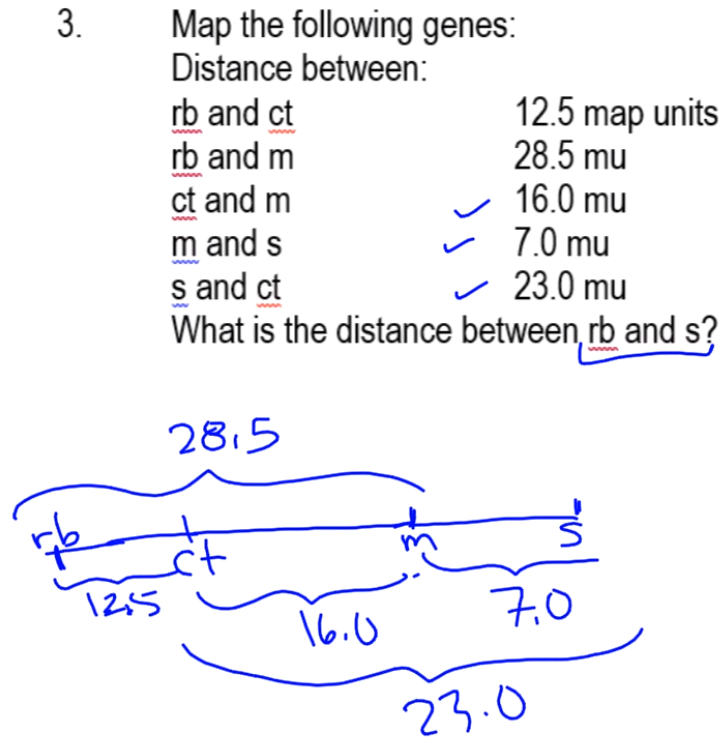
\includegraphics[width=0.5\textwidth]{mapping}
    \caption{rb $\longrightarrow$ ct $\longrightarrow$ m $\longrightarrow$ s}
\end{figure}

Answer: \SI{35.5}{mu} ($\SI{28.5}{mu} + \SI{7.0}{mu}$)

\subsection{Applications}
You don't really need to memorize this.

\subsubsection{Gene Insertion}
\begin{itemize}
    \item{Normal gene inserted into position on chromosome of a diseased cell}
\end{itemize}

\subsubsection{Gene Modification}
\begin{itemize}
    \item{Defective gene is modified chemically to recode genetic message}
\end{itemize}

\subsubsection{Gene Surgery}
\begin{itemize}
    \item{Defective gene is extracted}
    \item{Replaced with a normal gene}
\end{itemize}

\end{document}
